\chapter{Results}\label{chap:results}
\section{The Primary Goal - The Product}
The end result of the development resulted in a fully deployed system that enables the user to communicate with other users connecting to the same room. The user is able to connect to rooms with other users around the world. The connected users are able to move around a virtual space, connecting to other users near their avatar and the volume of other users voices is automatically adjusted to simulate a real life environment.

The system is deployed on a Kubernetes cluster handling the lifetime of the different services that encompasses the entire CoffeeBreak system. Multiple of these services are automatically scaled to fit whatever need the system might have depending on user traffic levels. The cluster is hosted on Google Kubernetes Engine, which handles the overall cluster operations, in addition to the external IP and TLS configuration. This allows the system to operate over HTTPS giving the user a secure access to the system. 

\section{The Secondary Goal - Performance}
In addition to the overall goal, performance was also tested between the two different solutions. The results indicate that the P2P solution is more heavily reliant on client side performance due to the client browser handling all connections to the other users, while the MRS solution splits the load more evenly between the server and client. These tests were originally done looking at the CPU load of the users browser when testing the P2P solution and looking both on the clients CPU load and node CPU load when testing the MRS solution. 

As described during the design session, the results should end with the P2P solution having a exponential growth in CPU consumption due to the exponential growth in user connections. Also, the MRS solution should result in a linear CPU usage growth due to the linear growth user connections. Below is two graphs illustrating this behavior after testing both designs on a local machine.

\begin{figure}[]
    \centering
    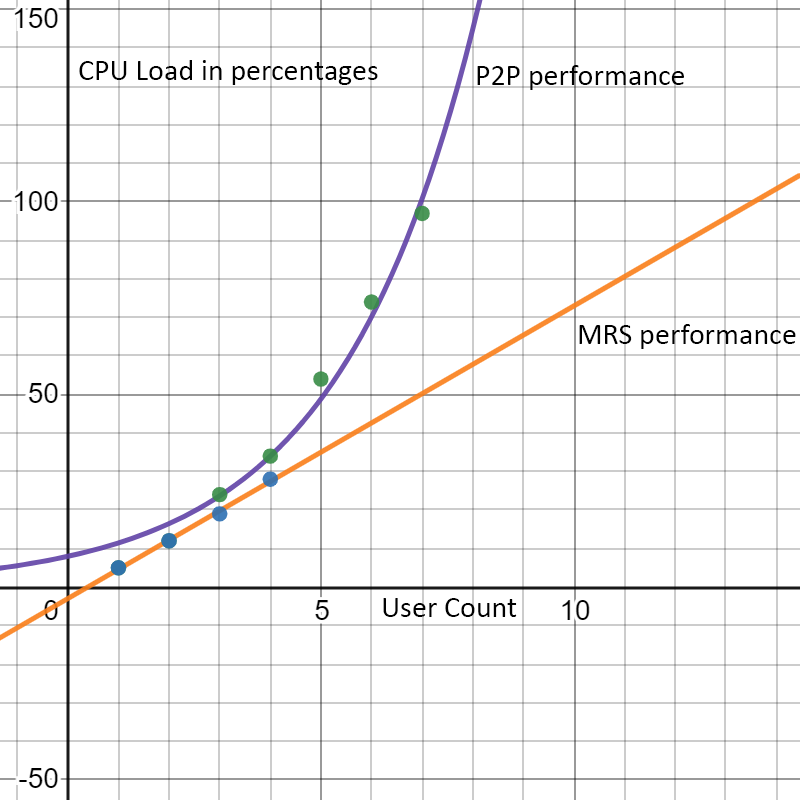
\includegraphics[width=0.65\textwidth]{Pictures/Performance Graph.png}
    \caption{Illustrates the the effect of CPU usage based on user count for both of the implemented solutions}
    \label{fig:performance-graph}
\end{figure}

\newpage

As illustrated above, the CPU usage increases exponentially with the P2P design, while it increases linear with the MRS design. This confirms the initial design assumptions.

Lastly, overall performance testing was also run on the overall cluster to stress test the deployment in high traffic situations. Through the use of Artillery, a number of stress tests was created to give insight into the overall system performance during high stress situations. Areas a such as Database read and write was tested through a influx of requests, rising in volume over a period of time. All tests resulted in a 99.99\% success. This shows that the system is capable of massive influx of connections. 

A rudimentary evaluation of technical complexity determines that the technical difficulty between implementing the twin designs is apparent by the number of system components alone. The Vili design has a total of seven components, one more than the Odin design, with that seventh component being of significant difficulty to implement due to the complexity of the involved technologies. Furthermore, the physical deployment of the system requires further miscellaneous changes to accommodate the media relay server. The team is confident in concluding that, while using a media relay server might have performance benefits, it does come with significant added development complexity, and is not worth doing unless necessary.

In addition to test the socket server, a stress test was created to simulate real users connection to the socket. These simulated users consists of three user archetypes. A "Lurker", which connects to the room and doesn't do anything, a "Quiet chatter", which sends a message once, and a "Frequent Chatter", which sends a message every second for twenty seconds. Running this test shows that many users are capable of joining the same room and the socket server can handle many connections simultaneously, without any connection problems and the horizontal pod auto-scalers spin new pods up when CPU usage reaches a certain milestone.

The full summary reports can be found in the appendix